\documentclass[twoside]{book}

% Packages required by doxygen
\usepackage{fixltx2e}
\usepackage{calc}
\usepackage{doxygen}
\usepackage[export]{adjustbox} % also loads graphicx
\usepackage{graphicx}
\usepackage[utf8]{inputenc}
\usepackage{makeidx}
\usepackage{multicol}
\usepackage{multirow}
\PassOptionsToPackage{warn}{textcomp}
\usepackage{textcomp}
\usepackage[nointegrals]{wasysym}
\usepackage[table]{xcolor}

% Font selection
\usepackage[T1]{fontenc}
\usepackage[scaled=.90]{helvet}
\usepackage{courier}
\usepackage{amssymb}
\usepackage{sectsty}
\renewcommand{\familydefault}{\sfdefault}
\allsectionsfont{%
  \fontseries{bc}\selectfont%
  \color{darkgray}%
}
\renewcommand{\DoxyLabelFont}{%
  \fontseries{bc}\selectfont%
  \color{darkgray}%
}
\newcommand{\+}{\discretionary{\mbox{\scriptsize$\hookleftarrow$}}{}{}}

% Page & text layout
\usepackage{geometry}
\geometry{%
  a4paper,%
  top=2.5cm,%
  bottom=2.5cm,%
  left=2.5cm,%
  right=2.5cm%
}
\tolerance=750
\hfuzz=15pt
\hbadness=750
\setlength{\emergencystretch}{15pt}
\setlength{\parindent}{0cm}
\setlength{\parskip}{3ex plus 2ex minus 2ex}
\makeatletter
\renewcommand{\paragraph}{%
  \@startsection{paragraph}{4}{0ex}{-1.0ex}{1.0ex}{%
    \normalfont\normalsize\bfseries\SS@parafont%
  }%
}
\renewcommand{\subparagraph}{%
  \@startsection{subparagraph}{5}{0ex}{-1.0ex}{1.0ex}{%
    \normalfont\normalsize\bfseries\SS@subparafont%
  }%
}
\makeatother

% Headers & footers
\usepackage{fancyhdr}
\pagestyle{fancyplain}
\fancyhead[LE]{\fancyplain{}{\bfseries\thepage}}
\fancyhead[CE]{\fancyplain{}{}}
\fancyhead[RE]{\fancyplain{}{\bfseries\leftmark}}
\fancyhead[LO]{\fancyplain{}{\bfseries\rightmark}}
\fancyhead[CO]{\fancyplain{}{}}
\fancyhead[RO]{\fancyplain{}{\bfseries\thepage}}
\fancyfoot[LE]{\fancyplain{}{}}
\fancyfoot[CE]{\fancyplain{}{}}
\fancyfoot[RE]{\fancyplain{}{\bfseries\scriptsize Generated by Doxygen }}
\fancyfoot[LO]{\fancyplain{}{\bfseries\scriptsize Generated by Doxygen }}
\fancyfoot[CO]{\fancyplain{}{}}
\fancyfoot[RO]{\fancyplain{}{}}
\renewcommand{\footrulewidth}{0.4pt}
\renewcommand{\chaptermark}[1]{%
  \markboth{#1}{}%
}
\renewcommand{\sectionmark}[1]{%
  \markright{\thesection\ #1}%
}

% Indices & bibliography
\usepackage{natbib}
\usepackage[titles]{tocloft}
\setcounter{tocdepth}{3}
\setcounter{secnumdepth}{5}
\makeindex

% Hyperlinks (required, but should be loaded last)
\usepackage{ifpdf}
\ifpdf
  \usepackage[pdftex,pagebackref=true]{hyperref}
\else
  \usepackage[ps2pdf,pagebackref=true]{hyperref}
\fi
\hypersetup{%
  colorlinks=true,%
  linkcolor=blue,%
  citecolor=blue,%
  unicode%
}

% Custom commands
\newcommand{\clearemptydoublepage}{%
  \newpage{\pagestyle{empty}\cleardoublepage}%
}

\usepackage{caption}
\captionsetup{labelsep=space,justification=centering,font={bf},singlelinecheck=off,skip=4pt,position=top}

%===== C O N T E N T S =====

\begin{document}

% Titlepage & ToC
\hypersetup{pageanchor=false,
             bookmarksnumbered=true,
             pdfencoding=unicode
            }
\pagenumbering{roman}
\begin{titlepage}
\vspace*{7cm}
\begin{center}%
{\Large D\+S\+M\+DE \\[1ex]\large 0.\+1 }\\
\vspace*{1cm}
{\large Generated by Doxygen 1.8.11}\\
\end{center}
\end{titlepage}
\clearemptydoublepage
\tableofcontents
\clearemptydoublepage
\pagenumbering{arabic}
\hypersetup{pageanchor=true}

%--- Begin generated contents ---
\chapter{Namespace Index}
\section{Packages}
Here are the packages with brief descriptions (if available)\+:\begin{DoxyCompactList}
\item\contentsline{section}{\hyperlink{namespacedriver}{driver} }{\pageref{namespacedriver}}{}
\item\contentsline{section}{\hyperlink{namespacescanner}{scanner} }{\pageref{namespacescanner}}{}
\end{DoxyCompactList}

\chapter{Hierarchical Index}
\section{Class Hierarchy}
This inheritance list is sorted roughly, but not completely, alphabetically\+:\begin{DoxyCompactList}
\item \contentsline{section}{driver.\+Administration}{\pageref{classdriver_1_1Administration}}{}
\item \contentsline{section}{driver.\+driver}{\pageref{classdriver_1_1driver}}{}
\item \contentsline{section}{parser.\+First\+Follow}{\pageref{classparser_1_1FirstFollow}}{}
\item \contentsline{section}{parser.\+Parser}{\pageref{classparser_1_1Parser}}{}
\item \contentsline{section}{scanner.\+Scan\+Me}{\pageref{classscanner_1_1ScanMe}}{}
\item \contentsline{section}{scanner.\+Symbol}{\pageref{enumscanner_1_1Symbol}}{}
\item \contentsline{section}{symbol\+Table.\+Symbol\+Table}{\pageref{classsymbolTable_1_1SymbolTable}}{}
\item \contentsline{section}{scanner.\+Token}{\pageref{classscanner_1_1Token}}{}
\item J\+Frame\begin{DoxyCompactList}
\item \contentsline{section}{driver.\+Driver\+Window}{\pageref{classdriver_1_1DriverWindow}}{}
\end{DoxyCompactList}
\end{DoxyCompactList}

\chapter{Class Index}
\section{Class List}
Here are the classes, structs, unions and interfaces with brief descriptions\+:\begin{DoxyCompactList}
\item\contentsline{section}{\hyperlink{classdriver_1_1driver}{driver.\+driver} }{\pageref{classdriver_1_1driver}}{}
\item\contentsline{section}{\hyperlink{classdriver_1_1DriverWindow}{driver.\+Driver\+Window} }{\pageref{classdriver_1_1DriverWindow}}{}
\item\contentsline{section}{\hyperlink{classscanner_1_1Scanner}{scanner.\+Scanner} }{\pageref{classscanner_1_1Scanner}}{}
\end{DoxyCompactList}

\chapter{File Index}
\section{File List}
Here is a list of all files with brief descriptions\+:\begin{DoxyCompactList}
\item\contentsline{section}{src/driver/\hyperlink{driver_8java}{driver.\+java} \\*Drives the project }{\pageref{driver_8java}}{}
\item\contentsline{section}{src/driver/\hyperlink{DriverWindow_8java}{Driver\+Window.\+java} \\*This the driver class Provides UI for user to choose file from dialog }{\pageref{DriverWindow_8java}}{}
\item\contentsline{section}{src/scanner/\hyperlink{Scanner_8java}{Scanner.\+java} \\*This the scanner class This class generates meaningful tokens from source file }{\pageref{Scanner_8java}}{}
\end{DoxyCompactList}

\chapter{Namespace Documentation}
\hypertarget{namespacedriver}{}\section{Package driver}
\label{namespacedriver}\index{driver@{driver}}
\subsection*{Classes}
\begin{DoxyCompactItemize}
\item 
class \hyperlink{classdriver_1_1Administration}{Administration}
\item 
class \hyperlink{classdriver_1_1driver}{driver}
\item 
class \hyperlink{classdriver_1_1DriverWindow}{Driver\+Window}
\end{DoxyCompactItemize}

\hypertarget{namespaceparser}{}\section{Package parser}
\label{namespaceparser}\index{parser@{parser}}
\subsection*{Classes}
\begin{DoxyCompactItemize}
\item 
class \hyperlink{classparser_1_1FirstFollow}{First\+Follow}
\item 
class \hyperlink{classparser_1_1Parser}{Parser}
\end{DoxyCompactItemize}

\hypertarget{namespacescanner}{}\section{Package scanner}
\label{namespacescanner}\index{scanner@{scanner}}
\subsection*{Classes}
\begin{DoxyCompactItemize}
\item 
class \hyperlink{classscanner_1_1ScanMe}{Scan\+Me}
\item 
enum \hyperlink{enumscanner_1_1Symbol}{Symbol}
\item 
class \hyperlink{classscanner_1_1Token}{Token}
\end{DoxyCompactItemize}

\hypertarget{namespacesymbolTable}{}\section{Package symbol\+Table}
\label{namespacesymbolTable}\index{symbol\+Table@{symbol\+Table}}
\subsection*{Classes}
\begin{DoxyCompactItemize}
\item 
class \hyperlink{classsymbolTable_1_1SymbolTable}{Symbol\+Table}
\end{DoxyCompactItemize}

\chapter{Class Documentation}
\hypertarget{classdriver_1_1Administration}{}\section{driver.\+Administration Class Reference}
\label{classdriver_1_1Administration}\index{driver.\+Administration@{driver.\+Administration}}
\subsection*{Public Member Functions}
\begin{DoxyCompactItemize}
\item 
\hyperlink{classdriver_1_1Administration_a1e378b8b16a9c1ef1970d4fbebad410b}{Administration} (\hyperlink{classscanner_1_1ScanMe}{Scan\+Me} sc, \hyperlink{classsymbolTable_1_1SymbolTable}{Symbol\+Table} st)
\item 
void \hyperlink{classdriver_1_1Administration_a38c447b6b2cb98af3ddaa006f0ea1d29}{start} ()
\item 
void \hyperlink{classdriver_1_1Administration_aec10ee76df416687adcc1ed8ddfbfd24}{New\+Line} ()
\item 
void \hyperlink{classdriver_1_1Administration_af0886dadf0168b179711af4acebc2307}{error} (int error\+Type, \hyperlink{enumscanner_1_1Symbol}{Symbol} sym, int flag)
\end{DoxyCompactItemize}
\subsection*{Public Attributes}
\begin{DoxyCompactItemize}
\item 
int \hyperlink{classdriver_1_1Administration_a89a69f2397f1fb011677557ffa1c64fc}{line\+No}
\end{DoxyCompactItemize}


\subsection{Constructor \& Destructor Documentation}
\index{driver\+::\+Administration@{driver\+::\+Administration}!Administration@{Administration}}
\index{Administration@{Administration}!driver\+::\+Administration@{driver\+::\+Administration}}
\subsubsection[{\texorpdfstring{Administration(\+Scan\+Me sc, Symbol\+Table st)}{Administration(ScanMe sc, SymbolTable st)}}]{\setlength{\rightskip}{0pt plus 5cm}driver.\+Administration.\+Administration (
\begin{DoxyParamCaption}
\item[{{\bf Scan\+Me}}]{sc, }
\item[{{\bf Symbol\+Table}}]{st}
\end{DoxyParamCaption}
)}\hypertarget{classdriver_1_1Administration_a1e378b8b16a9c1ef1970d4fbebad410b}{}\label{classdriver_1_1Administration_a1e378b8b16a9c1ef1970d4fbebad410b}


\subsection{Member Function Documentation}
\index{driver\+::\+Administration@{driver\+::\+Administration}!error@{error}}
\index{error@{error}!driver\+::\+Administration@{driver\+::\+Administration}}
\subsubsection[{\texorpdfstring{error(int error\+Type, Symbol sym, int flag)}{error(int errorType, Symbol sym, int flag)}}]{\setlength{\rightskip}{0pt plus 5cm}void driver.\+Administration.\+error (
\begin{DoxyParamCaption}
\item[{int}]{error\+Type, }
\item[{{\bf Symbol}}]{sym, }
\item[{int}]{flag}
\end{DoxyParamCaption}
)}\hypertarget{classdriver_1_1Administration_af0886dadf0168b179711af4acebc2307}{}\label{classdriver_1_1Administration_af0886dadf0168b179711af4acebc2307}
\index{driver\+::\+Administration@{driver\+::\+Administration}!New\+Line@{New\+Line}}
\index{New\+Line@{New\+Line}!driver\+::\+Administration@{driver\+::\+Administration}}
\subsubsection[{\texorpdfstring{New\+Line()}{NewLine()}}]{\setlength{\rightskip}{0pt plus 5cm}void driver.\+Administration.\+New\+Line (
\begin{DoxyParamCaption}
{}
\end{DoxyParamCaption}
)}\hypertarget{classdriver_1_1Administration_aec10ee76df416687adcc1ed8ddfbfd24}{}\label{classdriver_1_1Administration_aec10ee76df416687adcc1ed8ddfbfd24}
\index{driver\+::\+Administration@{driver\+::\+Administration}!start@{start}}
\index{start@{start}!driver\+::\+Administration@{driver\+::\+Administration}}
\subsubsection[{\texorpdfstring{start()}{start()}}]{\setlength{\rightskip}{0pt plus 5cm}void driver.\+Administration.\+start (
\begin{DoxyParamCaption}
{}
\end{DoxyParamCaption}
)}\hypertarget{classdriver_1_1Administration_a38c447b6b2cb98af3ddaa006f0ea1d29}{}\label{classdriver_1_1Administration_a38c447b6b2cb98af3ddaa006f0ea1d29}


\subsection{Member Data Documentation}
\index{driver\+::\+Administration@{driver\+::\+Administration}!line\+No@{line\+No}}
\index{line\+No@{line\+No}!driver\+::\+Administration@{driver\+::\+Administration}}
\subsubsection[{\texorpdfstring{line\+No}{lineNo}}]{\setlength{\rightskip}{0pt plus 5cm}int driver.\+Administration.\+line\+No}\hypertarget{classdriver_1_1Administration_a89a69f2397f1fb011677557ffa1c64fc}{}\label{classdriver_1_1Administration_a89a69f2397f1fb011677557ffa1c64fc}


The documentation for this class was generated from the following file\+:\begin{DoxyCompactItemize}
\item 
src/driver/\hyperlink{Administration_8java}{Administration.\+java}\end{DoxyCompactItemize}

\hypertarget{classdriver_1_1driver}{}\section{driver.\+driver Class Reference}
\label{classdriver_1_1driver}\index{driver.\+driver@{driver.\+driver}}
\subsection*{Static Public Member Functions}
\begin{DoxyCompactItemize}
\item 
static void \hyperlink{classdriver_1_1driver_ab4bbf6027065ef2d09f1e20f8346d2bf}{main} (String\mbox{[}$\,$\mbox{]} args)
\end{DoxyCompactItemize}
\subsection*{Public Attributes}
\begin{DoxyCompactItemize}
\item 
int \hyperlink{classdriver_1_1driver_a171341186cc3c3a33ce7f44a938d9bcd}{var}
\end{DoxyCompactItemize}


\subsection{Detailed Description}
This is the main file. Program starts from main file 

\subsection{Member Function Documentation}
\index{driver\+::driver@{driver\+::driver}!main@{main}}
\index{main@{main}!driver\+::driver@{driver\+::driver}}
\subsubsection[{\texorpdfstring{main(\+String[] args)}{main(String[] args)}}]{\setlength{\rightskip}{0pt plus 5cm}static void driver.\+driver.\+main (
\begin{DoxyParamCaption}
\item[{String\mbox{[}$\,$\mbox{]}}]{args}
\end{DoxyParamCaption}
)\hspace{0.3cm}{\ttfamily [static]}}\hypertarget{classdriver_1_1driver_ab4bbf6027065ef2d09f1e20f8346d2bf}{}\label{classdriver_1_1driver_ab4bbf6027065ef2d09f1e20f8346d2bf}

\begin{DoxyParams}{Parameters}
{\em args} & \\
\hline
\end{DoxyParams}


\subsection{Member Data Documentation}
\index{driver\+::driver@{driver\+::driver}!var@{var}}
\index{var@{var}!driver\+::driver@{driver\+::driver}}
\subsubsection[{\texorpdfstring{var}{var}}]{\setlength{\rightskip}{0pt plus 5cm}int driver.\+driver.\+var}\hypertarget{classdriver_1_1driver_a171341186cc3c3a33ce7f44a938d9bcd}{}\label{classdriver_1_1driver_a171341186cc3c3a33ce7f44a938d9bcd}
this is a variable 

The documentation for this class was generated from the following file\+:\begin{DoxyCompactItemize}
\item 
src/driver/\hyperlink{driver_8java}{driver.\+java}\end{DoxyCompactItemize}

\hypertarget{classdriver_1_1DriverWindow}{}\section{driver.\+Driver\+Window Class Reference}
\label{classdriver_1_1DriverWindow}\index{driver.\+Driver\+Window@{driver.\+Driver\+Window}}
Inheritance diagram for driver.\+Driver\+Window\+:\begin{figure}[H]
\begin{center}
\leavevmode
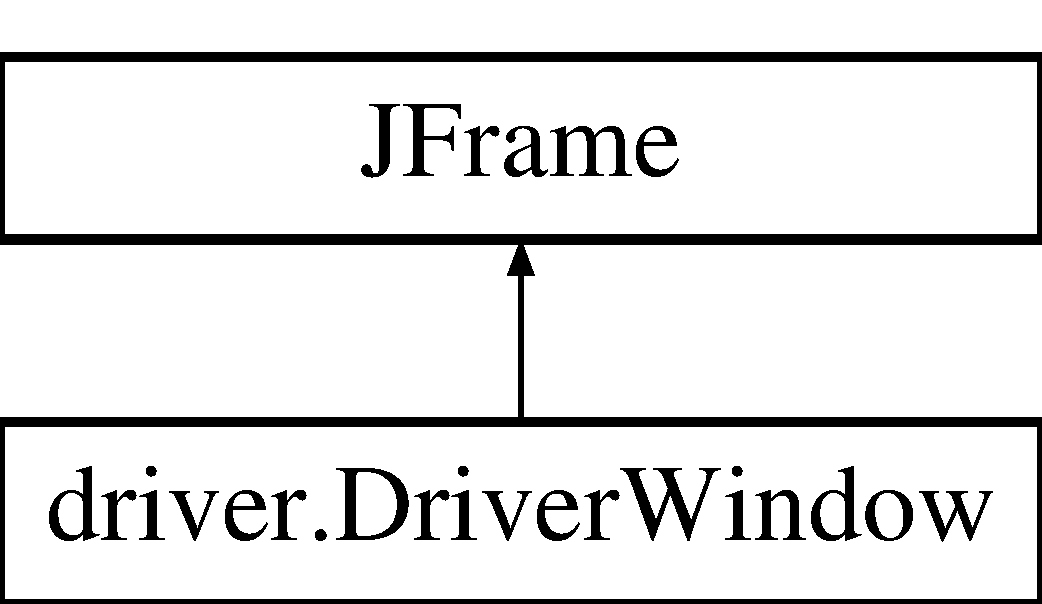
\includegraphics[height=2.000000cm]{classdriver_1_1DriverWindow}
\end{center}
\end{figure}
\subsection*{Public Member Functions}
\begin{DoxyCompactItemize}
\item 
\hyperlink{classdriver_1_1DriverWindow_acc35b31088a5ffe1543c28462b56194f}{Driver\+Window} ()
\end{DoxyCompactItemize}
\subsection*{Static Public Member Functions}
\begin{DoxyCompactItemize}
\item 
static void \hyperlink{classdriver_1_1DriverWindow_af743a70776a96562bbfb500b93a2e742}{main} (String\mbox{[}$\,$\mbox{]} args)
\end{DoxyCompactItemize}
\subsection*{Public Attributes}
\begin{DoxyCompactItemize}
\item 
File\+Reader \hyperlink{classdriver_1_1DriverWindow_a463a3d013ea4e8f95c818b2f7a7842d0}{source\+File} = null
\begin{DoxyCompactList}\small\item\em source\+File object is the reader of source file \end{DoxyCompactList}\end{DoxyCompactItemize}
\subsection*{Private Member Functions}
\begin{DoxyCompactItemize}
\item 
void \hyperlink{classdriver_1_1DriverWindow_a0513dffb45726e4a9ef3db30c3aec57e}{open\+File\+Stream} (String absolute\+Path)
\end{DoxyCompactItemize}
\subsection*{Private Attributes}
\begin{DoxyCompactItemize}
\item 
J\+Panel \hyperlink{classdriver_1_1DriverWindow_ac02788f4ca5e699895e910d672237baa}{content\+Pane}
\item 
J\+Text\+Field \hyperlink{classdriver_1_1DriverWindow_a28cd643f483a25f1793d57daae2813b1}{text\+Field}
\end{DoxyCompactItemize}


\subsection{Constructor \& Destructor Documentation}
\index{driver\+::\+Driver\+Window@{driver\+::\+Driver\+Window}!Driver\+Window@{Driver\+Window}}
\index{Driver\+Window@{Driver\+Window}!driver\+::\+Driver\+Window@{driver\+::\+Driver\+Window}}
\subsubsection[{\texorpdfstring{Driver\+Window()}{DriverWindow()}}]{\setlength{\rightskip}{0pt plus 5cm}driver.\+Driver\+Window.\+Driver\+Window (
\begin{DoxyParamCaption}
{}
\end{DoxyParamCaption}
)}\hypertarget{classdriver_1_1DriverWindow_acc35b31088a5ffe1543c28462b56194f}{}\label{classdriver_1_1DriverWindow_acc35b31088a5ffe1543c28462b56194f}
Create the frame. 

\subsection{Member Function Documentation}
\index{driver\+::\+Driver\+Window@{driver\+::\+Driver\+Window}!main@{main}}
\index{main@{main}!driver\+::\+Driver\+Window@{driver\+::\+Driver\+Window}}
\subsubsection[{\texorpdfstring{main(\+String[] args)}{main(String[] args)}}]{\setlength{\rightskip}{0pt plus 5cm}static void driver.\+Driver\+Window.\+main (
\begin{DoxyParamCaption}
\item[{String\mbox{[}$\,$\mbox{]}}]{args}
\end{DoxyParamCaption}
)\hspace{0.3cm}{\ttfamily [static]}}\hypertarget{classdriver_1_1DriverWindow_af743a70776a96562bbfb500b93a2e742}{}\label{classdriver_1_1DriverWindow_af743a70776a96562bbfb500b93a2e742}
Launch the application. \index{driver\+::\+Driver\+Window@{driver\+::\+Driver\+Window}!open\+File\+Stream@{open\+File\+Stream}}
\index{open\+File\+Stream@{open\+File\+Stream}!driver\+::\+Driver\+Window@{driver\+::\+Driver\+Window}}
\subsubsection[{\texorpdfstring{open\+File\+Stream(\+String absolute\+Path)}{openFileStream(String absolutePath)}}]{\setlength{\rightskip}{0pt plus 5cm}void driver.\+Driver\+Window.\+open\+File\+Stream (
\begin{DoxyParamCaption}
\item[{String}]{absolute\+Path}
\end{DoxyParamCaption}
)\hspace{0.3cm}{\ttfamily [private]}}\hypertarget{classdriver_1_1DriverWindow_a0513dffb45726e4a9ef3db30c3aec57e}{}\label{classdriver_1_1DriverWindow_a0513dffb45726e4a9ef3db30c3aec57e}

\begin{DoxyParams}{Parameters}
{\em absolute\+Path} & opens file using file reader and the absolute path of the chosen file \\
\hline
\end{DoxyParams}


\subsection{Member Data Documentation}
\index{driver\+::\+Driver\+Window@{driver\+::\+Driver\+Window}!content\+Pane@{content\+Pane}}
\index{content\+Pane@{content\+Pane}!driver\+::\+Driver\+Window@{driver\+::\+Driver\+Window}}
\subsubsection[{\texorpdfstring{content\+Pane}{contentPane}}]{\setlength{\rightskip}{0pt plus 5cm}J\+Panel driver.\+Driver\+Window.\+content\+Pane\hspace{0.3cm}{\ttfamily [private]}}\hypertarget{classdriver_1_1DriverWindow_ac02788f4ca5e699895e910d672237baa}{}\label{classdriver_1_1DriverWindow_ac02788f4ca5e699895e910d672237baa}
\index{driver\+::\+Driver\+Window@{driver\+::\+Driver\+Window}!source\+File@{source\+File}}
\index{source\+File@{source\+File}!driver\+::\+Driver\+Window@{driver\+::\+Driver\+Window}}
\subsubsection[{\texorpdfstring{source\+File}{sourceFile}}]{\setlength{\rightskip}{0pt plus 5cm}File\+Reader driver.\+Driver\+Window.\+source\+File = null}\hypertarget{classdriver_1_1DriverWindow_a463a3d013ea4e8f95c818b2f7a7842d0}{}\label{classdriver_1_1DriverWindow_a463a3d013ea4e8f95c818b2f7a7842d0}


source\+File object is the reader of source file 

\index{driver\+::\+Driver\+Window@{driver\+::\+Driver\+Window}!text\+Field@{text\+Field}}
\index{text\+Field@{text\+Field}!driver\+::\+Driver\+Window@{driver\+::\+Driver\+Window}}
\subsubsection[{\texorpdfstring{text\+Field}{textField}}]{\setlength{\rightskip}{0pt plus 5cm}J\+Text\+Field driver.\+Driver\+Window.\+text\+Field\hspace{0.3cm}{\ttfamily [private]}}\hypertarget{classdriver_1_1DriverWindow_a28cd643f483a25f1793d57daae2813b1}{}\label{classdriver_1_1DriverWindow_a28cd643f483a25f1793d57daae2813b1}


The documentation for this class was generated from the following file\+:\begin{DoxyCompactItemize}
\item 
src/driver/\hyperlink{DriverWindow_8java}{Driver\+Window.\+java}\end{DoxyCompactItemize}

\hypertarget{classparser_1_1FirstFollow}{}\section{parser.\+First\+Follow Class Reference}
\label{classparser_1_1FirstFollow}\index{parser.\+First\+Follow@{parser.\+First\+Follow}}


The documentation for this class was generated from the following file\+:\begin{DoxyCompactItemize}
\item 
src/parser/\hyperlink{FirstFollow_8java}{First\+Follow.\+java}\end{DoxyCompactItemize}

\hypertarget{classparser_1_1Parser}{}\section{parser.\+Parser Class Reference}
\label{classparser_1_1Parser}\index{parser.\+Parser@{parser.\+Parser}}
\subsection*{Public Member Functions}
\begin{DoxyCompactItemize}
\item 
\hyperlink{classparser_1_1Parser_aebdc8a7ecdcb71f2f174a01a31850e42}{Parser} (\hyperlink{classscanner_1_1ScanMe}{Scan\+Me} sc, \hyperlink{classdriver_1_1Administration}{Administration} ad)
\item 
void \hyperlink{classparser_1_1Parser_ad1f3cd238bb983941cd98449dfc8497f}{Dsmde\+Format} (\hyperlink{enumscanner_1_1Symbol}{Symbol} sym)
\end{DoxyCompactItemize}
\subsection*{Private Member Functions}
\begin{DoxyCompactItemize}
\item 
void \hyperlink{classparser_1_1Parser_abd40f2d896372bb3ecc2c1cc2acdf987}{Mod\+Element\+Names} (Vector$<$ \hyperlink{enumscanner_1_1Symbol}{Symbol} $>$ stops)
\item 
void \hyperlink{classparser_1_1Parser_a0ac8ad9d4539bf58428d64ff2c36bfa4}{Interact\+Attribute\+Names} (Vector$<$ \hyperlink{enumscanner_1_1Symbol}{Symbol} $>$ stops)
\item 
boolean \hyperlink{classparser_1_1Parser_a4fdc3423c8de027cc90e3ca6b34b6797}{in} (Vector$<$ \hyperlink{enumscanner_1_1Symbol}{Symbol} $>$ set)
\end{DoxyCompactItemize}


\subsection{Constructor \& Destructor Documentation}
\index{parser\+::\+Parser@{parser\+::\+Parser}!Parser@{Parser}}
\index{Parser@{Parser}!parser\+::\+Parser@{parser\+::\+Parser}}
\subsubsection[{\texorpdfstring{Parser(\+Scan\+Me sc, Administration ad)}{Parser(ScanMe sc, Administration ad)}}]{\setlength{\rightskip}{0pt plus 5cm}parser.\+Parser.\+Parser (
\begin{DoxyParamCaption}
\item[{{\bf Scan\+Me}}]{sc, }
\item[{{\bf Administration}}]{ad}
\end{DoxyParamCaption}
)}\hypertarget{classparser_1_1Parser_aebdc8a7ecdcb71f2f174a01a31850e42}{}\label{classparser_1_1Parser_aebdc8a7ecdcb71f2f174a01a31850e42}


\subsection{Member Function Documentation}
\index{parser\+::\+Parser@{parser\+::\+Parser}!Dsmde\+Format@{Dsmde\+Format}}
\index{Dsmde\+Format@{Dsmde\+Format}!parser\+::\+Parser@{parser\+::\+Parser}}
\subsubsection[{\texorpdfstring{Dsmde\+Format(\+Symbol sym)}{DsmdeFormat(Symbol sym)}}]{\setlength{\rightskip}{0pt plus 5cm}void parser.\+Parser.\+Dsmde\+Format (
\begin{DoxyParamCaption}
\item[{{\bf Symbol}}]{sym}
\end{DoxyParamCaption}
)}\hypertarget{classparser_1_1Parser_ad1f3cd238bb983941cd98449dfc8497f}{}\label{classparser_1_1Parser_ad1f3cd238bb983941cd98449dfc8497f}
\index{parser\+::\+Parser@{parser\+::\+Parser}!in@{in}}
\index{in@{in}!parser\+::\+Parser@{parser\+::\+Parser}}
\subsubsection[{\texorpdfstring{in(\+Vector$<$ Symbol $>$ set)}{in(Vector< Symbol > set)}}]{\setlength{\rightskip}{0pt plus 5cm}boolean parser.\+Parser.\+in (
\begin{DoxyParamCaption}
\item[{Vector$<$ {\bf Symbol} $>$}]{set}
\end{DoxyParamCaption}
)\hspace{0.3cm}{\ttfamily [private]}}\hypertarget{classparser_1_1Parser_a4fdc3423c8de027cc90e3ca6b34b6797}{}\label{classparser_1_1Parser_a4fdc3423c8de027cc90e3ca6b34b6797}
\index{parser\+::\+Parser@{parser\+::\+Parser}!Interact\+Attribute\+Names@{Interact\+Attribute\+Names}}
\index{Interact\+Attribute\+Names@{Interact\+Attribute\+Names}!parser\+::\+Parser@{parser\+::\+Parser}}
\subsubsection[{\texorpdfstring{Interact\+Attribute\+Names(\+Vector$<$ Symbol $>$ stops)}{InteractAttributeNames(Vector< Symbol > stops)}}]{\setlength{\rightskip}{0pt plus 5cm}void parser.\+Parser.\+Interact\+Attribute\+Names (
\begin{DoxyParamCaption}
\item[{Vector$<$ {\bf Symbol} $>$}]{stops}
\end{DoxyParamCaption}
)\hspace{0.3cm}{\ttfamily [private]}}\hypertarget{classparser_1_1Parser_a0ac8ad9d4539bf58428d64ff2c36bfa4}{}\label{classparser_1_1Parser_a0ac8ad9d4539bf58428d64ff2c36bfa4}
\index{parser\+::\+Parser@{parser\+::\+Parser}!Mod\+Element\+Names@{Mod\+Element\+Names}}
\index{Mod\+Element\+Names@{Mod\+Element\+Names}!parser\+::\+Parser@{parser\+::\+Parser}}
\subsubsection[{\texorpdfstring{Mod\+Element\+Names(\+Vector$<$ Symbol $>$ stops)}{ModElementNames(Vector< Symbol > stops)}}]{\setlength{\rightskip}{0pt plus 5cm}void parser.\+Parser.\+Mod\+Element\+Names (
\begin{DoxyParamCaption}
\item[{Vector$<$ {\bf Symbol} $>$}]{stops}
\end{DoxyParamCaption}
)\hspace{0.3cm}{\ttfamily [private]}}\hypertarget{classparser_1_1Parser_abd40f2d896372bb3ecc2c1cc2acdf987}{}\label{classparser_1_1Parser_abd40f2d896372bb3ecc2c1cc2acdf987}


The documentation for this class was generated from the following file\+:\begin{DoxyCompactItemize}
\item 
src/parser/\hyperlink{Parser_8java}{Parser.\+java}\end{DoxyCompactItemize}

\hypertarget{classscanner_1_1ScanMe}{}\section{scanner.\+Scan\+Me Class Reference}
\label{classscanner_1_1ScanMe}\index{scanner.\+Scan\+Me@{scanner.\+Scan\+Me}}
\subsection*{Public Member Functions}
\begin{DoxyCompactItemize}
\item 
\hyperlink{classscanner_1_1ScanMe_ac0e4d99c570ec7cd861e401bc3a17ee9}{Scan\+Me} (File\+Reader src\+File, \hyperlink{classsymbolTable_1_1SymbolTable}{Symbol\+Table} st)
\item 
\hyperlink{classscanner_1_1Token}{Token} \hyperlink{classscanner_1_1ScanMe_ad41c3ea7020d63b8ffc53541a82cbd9d}{next\+Token} ()
\item 
String \hyperlink{classscanner_1_1ScanMe_a04ba391917868707ec9646723e92228f}{next\+Text\+Line} ()
\item 
void \hyperlink{classscanner_1_1ScanMe_a8e01be637964978892726c2081588e54}{read} ()
\end{DoxyCompactItemize}


\subsection{Constructor \& Destructor Documentation}
\index{scanner\+::\+Scan\+Me@{scanner\+::\+Scan\+Me}!Scan\+Me@{Scan\+Me}}
\index{Scan\+Me@{Scan\+Me}!scanner\+::\+Scan\+Me@{scanner\+::\+Scan\+Me}}
\subsubsection[{\texorpdfstring{Scan\+Me(\+File\+Reader src\+File, Symbol\+Table st)}{ScanMe(FileReader srcFile, SymbolTable st)}}]{\setlength{\rightskip}{0pt plus 5cm}scanner.\+Scan\+Me.\+Scan\+Me (
\begin{DoxyParamCaption}
\item[{File\+Reader}]{src\+File, }
\item[{{\bf Symbol\+Table}}]{st}
\end{DoxyParamCaption}
)}\hypertarget{classscanner_1_1ScanMe_ac0e4d99c570ec7cd861e401bc3a17ee9}{}\label{classscanner_1_1ScanMe_ac0e4d99c570ec7cd861e401bc3a17ee9}
constructor 
\begin{DoxyParams}{Parameters}
{\em src\+File} & \\
\hline
\end{DoxyParams}


\subsection{Member Function Documentation}
\index{scanner\+::\+Scan\+Me@{scanner\+::\+Scan\+Me}!next\+Text\+Line@{next\+Text\+Line}}
\index{next\+Text\+Line@{next\+Text\+Line}!scanner\+::\+Scan\+Me@{scanner\+::\+Scan\+Me}}
\subsubsection[{\texorpdfstring{next\+Text\+Line()}{nextTextLine()}}]{\setlength{\rightskip}{0pt plus 5cm}String scanner.\+Scan\+Me.\+next\+Text\+Line (
\begin{DoxyParamCaption}
{}
\end{DoxyParamCaption}
)}\hypertarget{classscanner_1_1ScanMe_a04ba391917868707ec9646723e92228f}{}\label{classscanner_1_1ScanMe_a04ba391917868707ec9646723e92228f}
\index{scanner\+::\+Scan\+Me@{scanner\+::\+Scan\+Me}!next\+Token@{next\+Token}}
\index{next\+Token@{next\+Token}!scanner\+::\+Scan\+Me@{scanner\+::\+Scan\+Me}}
\subsubsection[{\texorpdfstring{next\+Token()}{nextToken()}}]{\setlength{\rightskip}{0pt plus 5cm}{\bf Token} scanner.\+Scan\+Me.\+next\+Token (
\begin{DoxyParamCaption}
{}
\end{DoxyParamCaption}
)}\hypertarget{classscanner_1_1ScanMe_ad41c3ea7020d63b8ffc53541a82cbd9d}{}\label{classscanner_1_1ScanMe_ad41c3ea7020d63b8ffc53541a82cbd9d}
\begin{DoxyReturn}{Returns}
token as enum \hyperlink{enumscanner_1_1Symbol}{Symbol} 
\end{DoxyReturn}
\index{scanner\+::\+Scan\+Me@{scanner\+::\+Scan\+Me}!read@{read}}
\index{read@{read}!scanner\+::\+Scan\+Me@{scanner\+::\+Scan\+Me}}
\subsubsection[{\texorpdfstring{read()}{read()}}]{\setlength{\rightskip}{0pt plus 5cm}void scanner.\+Scan\+Me.\+read (
\begin{DoxyParamCaption}
{}
\end{DoxyParamCaption}
)}\hypertarget{classscanner_1_1ScanMe_a8e01be637964978892726c2081588e54}{}\label{classscanner_1_1ScanMe_a8e01be637964978892726c2081588e54}


The documentation for this class was generated from the following file\+:\begin{DoxyCompactItemize}
\item 
src/scanner/\hyperlink{ScanMe_8java}{Scan\+Me.\+java}\end{DoxyCompactItemize}

\hypertarget{enumscanner_1_1Symbol}{}\section{scanner.\+Symbol Enum Reference}
\label{enumscanner_1_1Symbol}\index{scanner.\+Symbol@{scanner.\+Symbol}}
\subsection*{Public Member Functions}
\begin{DoxyCompactItemize}
\item 
\hyperlink{enumscanner_1_1Symbol_a8ef20323663bc7edab38563a6d4a5318}{Symbol} (int \hyperlink{enumscanner_1_1Symbol_acf9fa625e4d4be91bcb93f6edef7d119}{code}, String lex)
\item 
int \hyperlink{enumscanner_1_1Symbol_ad0bfa41d4413bae1e046812633c59e6a}{get\+Code} ()
\item 
String \hyperlink{enumscanner_1_1Symbol_ae986ae2ce7a07522a8ea6a49beace3b2}{get\+Lexeme} ()
\end{DoxyCompactItemize}
\subsection*{Public Attributes}
\begin{DoxyCompactItemize}
\item 
\hyperlink{enumscanner_1_1Symbol_af4fb1e091459c3690d75e935cedf9a0c}{MM} =(256,\char`\"{}\%\%Matrix\+Market\char`\"{})
\item 
\hyperlink{enumscanner_1_1Symbol_ad4e8096b9d2c15f7a60ab047f4775587}{M\+A\+T\+R\+IX} =(257,\char`\"{}Matrix\char`\"{})
\item 
\hyperlink{enumscanner_1_1Symbol_ab0feed5b9424b0e1b51e308b308ad5a4}{D\+SM} =(258,\char`\"{}D\+SM\char`\"{})
\item 
\hyperlink{enumscanner_1_1Symbol_a81c78a2d8a9cc8251b277daba3086f37}{M\+DM} =(259,\char`\"{}M\+DM\char`\"{})
\item 
\hyperlink{enumscanner_1_1Symbol_ab0d045eb60ad3ff556028fb77fafe808}{D\+MM} =(260,\char`\"{}D\+MM\char`\"{})
\item 
\hyperlink{enumscanner_1_1Symbol_a4b0a4728ba24bbaa59681fc3846f4ccb}{C\+O\+O\+RD} =(261,\char`\"{}Coordinate\char`\"{})
\item 
\hyperlink{enumscanner_1_1Symbol_ab1c516201ec260d71a5127db4bd31ba1}{A\+R\+R\+AY} =(262,\char`\"{}Array\char`\"{})
\item 
\hyperlink{enumscanner_1_1Symbol_a834e51bc001411d99f5c903941982b10}{I\+NT} =(263,\char`\"{}Integer\char`\"{})
\item 
\hyperlink{enumscanner_1_1Symbol_add6a5347584a401c1af01fce41f59a4d}{R\+E\+AL} =(264,\char`\"{}Real\char`\"{})
\item 
\hyperlink{enumscanner_1_1Symbol_a3a17094f3037fbbbbeb7167b341f93d0}{C\+O\+M\+P\+L\+EX} =(265,\char`\"{}Complex\char`\"{})
\item 
\hyperlink{enumscanner_1_1Symbol_a30afa7ce84ee23d7012d3bbbc19c2134}{P\+A\+T\+T\+E\+RN} =(266,\char`\"{}Pattern\char`\"{})
\item 
\hyperlink{enumscanner_1_1Symbol_a655847fe3017a32515ceba8421e1e299}{G\+E\+N\+E\+R\+AL} =(267,\char`\"{}General\char`\"{})
\item 
\hyperlink{enumscanner_1_1Symbol_addfd36caed0aa6a5671258b44f1343f3}{S\+Y\+M\+E\+T\+R\+IC} =(268,\char`\"{}Symmetric\char`\"{})
\item 
\hyperlink{enumscanner_1_1Symbol_ac3fb066b62b3749077e8928786cd787a}{S\+K\+S\+Y\+M\+E\+T\+R\+IC} =(269,\char`\"{}Skew-\/Symmetric\textquotesingle{}\char`\"{})
\item 
\hyperlink{enumscanner_1_1Symbol_a54ab77d92fe2bc431bb8cb92f14ba893}{H\+E\+R\+M\+I\+T\+I\+AN} =(270,\char`\"{}Hermitian\char`\"{})
\item 
\hyperlink{enumscanner_1_1Symbol_adb3e5570967fd92fdd1954271afb106c}{IC} =(271,\char`\"{}IC\char`\"{})
\item 
\hyperlink{enumscanner_1_1Symbol_a8ab6664f58cbcb2473d37cbf9f60e926}{IR} =(272,\char`\"{}IR\char`\"{})
\item 
\hyperlink{enumscanner_1_1Symbol_ad6a62d8f6ff4dd72050d185f5ca284c4}{B\+D\+O\+M\+A\+IN} =(273,\char`\"{}\%begin\+Domain\char`\"{})
\item 
\hyperlink{enumscanner_1_1Symbol_ab42cf3cf57d25fb744a5dd5c9b63efc0}{E\+D\+O\+M\+A\+IN} =(274,\char`\"{}\%end\+Domain\char`\"{})
\item 
\hyperlink{enumscanner_1_1Symbol_a317540ed6fa5dd2a2d88bd2330f7885e}{B\+M\+O\+DE} =(275,\char`\"{}\%begin\+Mod\+Element\char`\"{})
\item 
\hyperlink{enumscanner_1_1Symbol_a2a421181e2f0e1c90ad0af595b6d8906}{E\+M\+O\+DE} =(276,\char`\"{}\%end\+Mod\+Element\char`\"{})
\item 
\hyperlink{enumscanner_1_1Symbol_a21607964d906cfc67cdb6d390919582b}{B\+A\+T\+T\+R\+IB} =(277,\char`\"{}\%begin\+Attribute\char`\"{})
\item 
\hyperlink{enumscanner_1_1Symbol_a78962cb98ddfb1e8e79c98f15c8f9643}{E\+A\+T\+T\+R\+IB} =(278,\char`\"{}\%end\+Attribute\char`\"{})
\item 
\hyperlink{enumscanner_1_1Symbol_a075212527a8bc8fba4907c4ba145107c}{C\+O\+M\+M\+E\+NT} =(279,\char`\"{}text\+Line\char`\"{})
\item 
\hyperlink{enumscanner_1_1Symbol_a5a82a1f927213af69169e22ee476fb55}{P\+L\+US} =(280,\char`\"{}+\char`\"{})
\item 
\hyperlink{enumscanner_1_1Symbol_ae7009205b3c1f781e1c88cb6009014ee}{M\+I\+N\+US} =(281,\char`\"{}-\/\char`\"{})
\item 
\hyperlink{enumscanner_1_1Symbol_a3fad7a9d1d48519d127a14c45c99b454}{E} =(282,\char`\"{}e\char`\"{})
\item 
\hyperlink{enumscanner_1_1Symbol_a42d90226a1f976a89daa673b88190c90}{N\+U\+M\+I\+NT} =(283,\char`\"{}num int\char`\"{})
\item 
\hyperlink{enumscanner_1_1Symbol_a4e4020d97e79ccd98f754f89e3017c1b}{N\+U\+M\+D\+O\+U\+B\+LE} =(284,\char`\"{}num double\char`\"{})
\item 
\hyperlink{enumscanner_1_1Symbol_ae8c4e968871042412d500b3278dcfda8}{U\+N\+D\+E\+F\+I\+N\+ED} =(285,\char`\"{}Undefined\char`\"{})
\item 
\hyperlink{enumscanner_1_1Symbol_a112ac5700480cd0695f81e027783a4e7}{E\+OF} =(286,\char`\"{}End of File\char`\"{})
\item 
\hyperlink{enumscanner_1_1Symbol_a824180c457dac27d762c237c0826520e}{N\+E\+W\+L\+I\+NE} =(287,\char`\"{}new line\char`\"{})
\end{DoxyCompactItemize}
\subsection*{Private Attributes}
\begin{DoxyCompactItemize}
\item 
final int \hyperlink{enumscanner_1_1Symbol_acf9fa625e4d4be91bcb93f6edef7d119}{code}
\item 
final String \hyperlink{enumscanner_1_1Symbol_a9039c6af68581d7c2c9ad2c9045f419f}{lexeme}
\end{DoxyCompactItemize}


\subsection{Constructor \& Destructor Documentation}
\index{scanner\+::\+Symbol@{scanner\+::\+Symbol}!Symbol@{Symbol}}
\index{Symbol@{Symbol}!scanner\+::\+Symbol@{scanner\+::\+Symbol}}
\subsubsection[{\texorpdfstring{Symbol(int code, String lex)}{Symbol(int code, String lex)}}]{\setlength{\rightskip}{0pt plus 5cm}scanner.\+Symbol.\+Symbol (
\begin{DoxyParamCaption}
\item[{int}]{code, }
\item[{String}]{lex}
\end{DoxyParamCaption}
)}\hypertarget{enumscanner_1_1Symbol_a8ef20323663bc7edab38563a6d4a5318}{}\label{enumscanner_1_1Symbol_a8ef20323663bc7edab38563a6d4a5318}


\subsection{Member Function Documentation}
\index{scanner\+::\+Symbol@{scanner\+::\+Symbol}!get\+Code@{get\+Code}}
\index{get\+Code@{get\+Code}!scanner\+::\+Symbol@{scanner\+::\+Symbol}}
\subsubsection[{\texorpdfstring{get\+Code()}{getCode()}}]{\setlength{\rightskip}{0pt plus 5cm}int scanner.\+Symbol.\+get\+Code (
\begin{DoxyParamCaption}
{}
\end{DoxyParamCaption}
)}\hypertarget{enumscanner_1_1Symbol_ad0bfa41d4413bae1e046812633c59e6a}{}\label{enumscanner_1_1Symbol_ad0bfa41d4413bae1e046812633c59e6a}
\index{scanner\+::\+Symbol@{scanner\+::\+Symbol}!get\+Lexeme@{get\+Lexeme}}
\index{get\+Lexeme@{get\+Lexeme}!scanner\+::\+Symbol@{scanner\+::\+Symbol}}
\subsubsection[{\texorpdfstring{get\+Lexeme()}{getLexeme()}}]{\setlength{\rightskip}{0pt plus 5cm}String scanner.\+Symbol.\+get\+Lexeme (
\begin{DoxyParamCaption}
{}
\end{DoxyParamCaption}
)}\hypertarget{enumscanner_1_1Symbol_ae986ae2ce7a07522a8ea6a49beace3b2}{}\label{enumscanner_1_1Symbol_ae986ae2ce7a07522a8ea6a49beace3b2}


\subsection{Member Data Documentation}
\index{scanner\+::\+Symbol@{scanner\+::\+Symbol}!A\+R\+R\+AY@{A\+R\+R\+AY}}
\index{A\+R\+R\+AY@{A\+R\+R\+AY}!scanner\+::\+Symbol@{scanner\+::\+Symbol}}
\subsubsection[{\texorpdfstring{A\+R\+R\+AY}{ARRAY}}]{\setlength{\rightskip}{0pt plus 5cm}scanner.\+Symbol.\+A\+R\+R\+AY =(262,\char`\"{}Array\char`\"{})}\hypertarget{enumscanner_1_1Symbol_ab1c516201ec260d71a5127db4bd31ba1}{}\label{enumscanner_1_1Symbol_ab1c516201ec260d71a5127db4bd31ba1}
\index{scanner\+::\+Symbol@{scanner\+::\+Symbol}!B\+A\+T\+T\+R\+IB@{B\+A\+T\+T\+R\+IB}}
\index{B\+A\+T\+T\+R\+IB@{B\+A\+T\+T\+R\+IB}!scanner\+::\+Symbol@{scanner\+::\+Symbol}}
\subsubsection[{\texorpdfstring{B\+A\+T\+T\+R\+IB}{BATTRIB}}]{\setlength{\rightskip}{0pt plus 5cm}scanner.\+Symbol.\+B\+A\+T\+T\+R\+IB =(277,\char`\"{}\%begin\+Attribute\char`\"{})}\hypertarget{enumscanner_1_1Symbol_a21607964d906cfc67cdb6d390919582b}{}\label{enumscanner_1_1Symbol_a21607964d906cfc67cdb6d390919582b}
\index{scanner\+::\+Symbol@{scanner\+::\+Symbol}!B\+D\+O\+M\+A\+IN@{B\+D\+O\+M\+A\+IN}}
\index{B\+D\+O\+M\+A\+IN@{B\+D\+O\+M\+A\+IN}!scanner\+::\+Symbol@{scanner\+::\+Symbol}}
\subsubsection[{\texorpdfstring{B\+D\+O\+M\+A\+IN}{BDOMAIN}}]{\setlength{\rightskip}{0pt plus 5cm}scanner.\+Symbol.\+B\+D\+O\+M\+A\+IN =(273,\char`\"{}\%begin\+Domain\char`\"{})}\hypertarget{enumscanner_1_1Symbol_ad6a62d8f6ff4dd72050d185f5ca284c4}{}\label{enumscanner_1_1Symbol_ad6a62d8f6ff4dd72050d185f5ca284c4}
\index{scanner\+::\+Symbol@{scanner\+::\+Symbol}!B\+M\+O\+DE@{B\+M\+O\+DE}}
\index{B\+M\+O\+DE@{B\+M\+O\+DE}!scanner\+::\+Symbol@{scanner\+::\+Symbol}}
\subsubsection[{\texorpdfstring{B\+M\+O\+DE}{BMODE}}]{\setlength{\rightskip}{0pt plus 5cm}scanner.\+Symbol.\+B\+M\+O\+DE =(275,\char`\"{}\%begin\+Mod\+Element\char`\"{})}\hypertarget{enumscanner_1_1Symbol_a317540ed6fa5dd2a2d88bd2330f7885e}{}\label{enumscanner_1_1Symbol_a317540ed6fa5dd2a2d88bd2330f7885e}
\index{scanner\+::\+Symbol@{scanner\+::\+Symbol}!code@{code}}
\index{code@{code}!scanner\+::\+Symbol@{scanner\+::\+Symbol}}
\subsubsection[{\texorpdfstring{code}{code}}]{\setlength{\rightskip}{0pt plus 5cm}final int scanner.\+Symbol.\+code\hspace{0.3cm}{\ttfamily [private]}}\hypertarget{enumscanner_1_1Symbol_acf9fa625e4d4be91bcb93f6edef7d119}{}\label{enumscanner_1_1Symbol_acf9fa625e4d4be91bcb93f6edef7d119}
\index{scanner\+::\+Symbol@{scanner\+::\+Symbol}!C\+O\+M\+M\+E\+NT@{C\+O\+M\+M\+E\+NT}}
\index{C\+O\+M\+M\+E\+NT@{C\+O\+M\+M\+E\+NT}!scanner\+::\+Symbol@{scanner\+::\+Symbol}}
\subsubsection[{\texorpdfstring{C\+O\+M\+M\+E\+NT}{COMMENT}}]{\setlength{\rightskip}{0pt plus 5cm}scanner.\+Symbol.\+C\+O\+M\+M\+E\+NT =(279,\char`\"{}text\+Line\char`\"{})}\hypertarget{enumscanner_1_1Symbol_a075212527a8bc8fba4907c4ba145107c}{}\label{enumscanner_1_1Symbol_a075212527a8bc8fba4907c4ba145107c}
\index{scanner\+::\+Symbol@{scanner\+::\+Symbol}!C\+O\+M\+P\+L\+EX@{C\+O\+M\+P\+L\+EX}}
\index{C\+O\+M\+P\+L\+EX@{C\+O\+M\+P\+L\+EX}!scanner\+::\+Symbol@{scanner\+::\+Symbol}}
\subsubsection[{\texorpdfstring{C\+O\+M\+P\+L\+EX}{COMPLEX}}]{\setlength{\rightskip}{0pt plus 5cm}scanner.\+Symbol.\+C\+O\+M\+P\+L\+EX =(265,\char`\"{}Complex\char`\"{})}\hypertarget{enumscanner_1_1Symbol_a3a17094f3037fbbbbeb7167b341f93d0}{}\label{enumscanner_1_1Symbol_a3a17094f3037fbbbbeb7167b341f93d0}
\index{scanner\+::\+Symbol@{scanner\+::\+Symbol}!C\+O\+O\+RD@{C\+O\+O\+RD}}
\index{C\+O\+O\+RD@{C\+O\+O\+RD}!scanner\+::\+Symbol@{scanner\+::\+Symbol}}
\subsubsection[{\texorpdfstring{C\+O\+O\+RD}{COORD}}]{\setlength{\rightskip}{0pt plus 5cm}scanner.\+Symbol.\+C\+O\+O\+RD =(261,\char`\"{}Coordinate\char`\"{})}\hypertarget{enumscanner_1_1Symbol_a4b0a4728ba24bbaa59681fc3846f4ccb}{}\label{enumscanner_1_1Symbol_a4b0a4728ba24bbaa59681fc3846f4ccb}
\index{scanner\+::\+Symbol@{scanner\+::\+Symbol}!D\+MM@{D\+MM}}
\index{D\+MM@{D\+MM}!scanner\+::\+Symbol@{scanner\+::\+Symbol}}
\subsubsection[{\texorpdfstring{D\+MM}{DMM}}]{\setlength{\rightskip}{0pt plus 5cm}scanner.\+Symbol.\+D\+MM =(260,\char`\"{}D\+MM\char`\"{})}\hypertarget{enumscanner_1_1Symbol_ab0d045eb60ad3ff556028fb77fafe808}{}\label{enumscanner_1_1Symbol_ab0d045eb60ad3ff556028fb77fafe808}
\index{scanner\+::\+Symbol@{scanner\+::\+Symbol}!D\+SM@{D\+SM}}
\index{D\+SM@{D\+SM}!scanner\+::\+Symbol@{scanner\+::\+Symbol}}
\subsubsection[{\texorpdfstring{D\+SM}{DSM}}]{\setlength{\rightskip}{0pt plus 5cm}scanner.\+Symbol.\+D\+SM =(258,\char`\"{}D\+SM\char`\"{})}\hypertarget{enumscanner_1_1Symbol_ab0feed5b9424b0e1b51e308b308ad5a4}{}\label{enumscanner_1_1Symbol_ab0feed5b9424b0e1b51e308b308ad5a4}
\index{scanner\+::\+Symbol@{scanner\+::\+Symbol}!E@{E}}
\index{E@{E}!scanner\+::\+Symbol@{scanner\+::\+Symbol}}
\subsubsection[{\texorpdfstring{E}{E}}]{\setlength{\rightskip}{0pt plus 5cm}scanner.\+Symbol.\+E =(282,\char`\"{}e\char`\"{})}\hypertarget{enumscanner_1_1Symbol_a3fad7a9d1d48519d127a14c45c99b454}{}\label{enumscanner_1_1Symbol_a3fad7a9d1d48519d127a14c45c99b454}
\index{scanner\+::\+Symbol@{scanner\+::\+Symbol}!E\+A\+T\+T\+R\+IB@{E\+A\+T\+T\+R\+IB}}
\index{E\+A\+T\+T\+R\+IB@{E\+A\+T\+T\+R\+IB}!scanner\+::\+Symbol@{scanner\+::\+Symbol}}
\subsubsection[{\texorpdfstring{E\+A\+T\+T\+R\+IB}{EATTRIB}}]{\setlength{\rightskip}{0pt plus 5cm}scanner.\+Symbol.\+E\+A\+T\+T\+R\+IB =(278,\char`\"{}\%end\+Attribute\char`\"{})}\hypertarget{enumscanner_1_1Symbol_a78962cb98ddfb1e8e79c98f15c8f9643}{}\label{enumscanner_1_1Symbol_a78962cb98ddfb1e8e79c98f15c8f9643}
\index{scanner\+::\+Symbol@{scanner\+::\+Symbol}!E\+D\+O\+M\+A\+IN@{E\+D\+O\+M\+A\+IN}}
\index{E\+D\+O\+M\+A\+IN@{E\+D\+O\+M\+A\+IN}!scanner\+::\+Symbol@{scanner\+::\+Symbol}}
\subsubsection[{\texorpdfstring{E\+D\+O\+M\+A\+IN}{EDOMAIN}}]{\setlength{\rightskip}{0pt plus 5cm}scanner.\+Symbol.\+E\+D\+O\+M\+A\+IN =(274,\char`\"{}\%end\+Domain\char`\"{})}\hypertarget{enumscanner_1_1Symbol_ab42cf3cf57d25fb744a5dd5c9b63efc0}{}\label{enumscanner_1_1Symbol_ab42cf3cf57d25fb744a5dd5c9b63efc0}
\index{scanner\+::\+Symbol@{scanner\+::\+Symbol}!E\+M\+O\+DE@{E\+M\+O\+DE}}
\index{E\+M\+O\+DE@{E\+M\+O\+DE}!scanner\+::\+Symbol@{scanner\+::\+Symbol}}
\subsubsection[{\texorpdfstring{E\+M\+O\+DE}{EMODE}}]{\setlength{\rightskip}{0pt plus 5cm}scanner.\+Symbol.\+E\+M\+O\+DE =(276,\char`\"{}\%end\+Mod\+Element\char`\"{})}\hypertarget{enumscanner_1_1Symbol_a2a421181e2f0e1c90ad0af595b6d8906}{}\label{enumscanner_1_1Symbol_a2a421181e2f0e1c90ad0af595b6d8906}
\index{scanner\+::\+Symbol@{scanner\+::\+Symbol}!E\+OF@{E\+OF}}
\index{E\+OF@{E\+OF}!scanner\+::\+Symbol@{scanner\+::\+Symbol}}
\subsubsection[{\texorpdfstring{E\+OF}{EOF}}]{\setlength{\rightskip}{0pt plus 5cm}scanner.\+Symbol.\+E\+OF =(286,\char`\"{}End of File\char`\"{})}\hypertarget{enumscanner_1_1Symbol_a112ac5700480cd0695f81e027783a4e7}{}\label{enumscanner_1_1Symbol_a112ac5700480cd0695f81e027783a4e7}
\index{scanner\+::\+Symbol@{scanner\+::\+Symbol}!G\+E\+N\+E\+R\+AL@{G\+E\+N\+E\+R\+AL}}
\index{G\+E\+N\+E\+R\+AL@{G\+E\+N\+E\+R\+AL}!scanner\+::\+Symbol@{scanner\+::\+Symbol}}
\subsubsection[{\texorpdfstring{G\+E\+N\+E\+R\+AL}{GENERAL}}]{\setlength{\rightskip}{0pt plus 5cm}scanner.\+Symbol.\+G\+E\+N\+E\+R\+AL =(267,\char`\"{}General\char`\"{})}\hypertarget{enumscanner_1_1Symbol_a655847fe3017a32515ceba8421e1e299}{}\label{enumscanner_1_1Symbol_a655847fe3017a32515ceba8421e1e299}
\index{scanner\+::\+Symbol@{scanner\+::\+Symbol}!H\+E\+R\+M\+I\+T\+I\+AN@{H\+E\+R\+M\+I\+T\+I\+AN}}
\index{H\+E\+R\+M\+I\+T\+I\+AN@{H\+E\+R\+M\+I\+T\+I\+AN}!scanner\+::\+Symbol@{scanner\+::\+Symbol}}
\subsubsection[{\texorpdfstring{H\+E\+R\+M\+I\+T\+I\+AN}{HERMITIAN}}]{\setlength{\rightskip}{0pt plus 5cm}scanner.\+Symbol.\+H\+E\+R\+M\+I\+T\+I\+AN =(270,\char`\"{}Hermitian\char`\"{})}\hypertarget{enumscanner_1_1Symbol_a54ab77d92fe2bc431bb8cb92f14ba893}{}\label{enumscanner_1_1Symbol_a54ab77d92fe2bc431bb8cb92f14ba893}
\index{scanner\+::\+Symbol@{scanner\+::\+Symbol}!IC@{IC}}
\index{IC@{IC}!scanner\+::\+Symbol@{scanner\+::\+Symbol}}
\subsubsection[{\texorpdfstring{IC}{IC}}]{\setlength{\rightskip}{0pt plus 5cm}scanner.\+Symbol.\+IC =(271,\char`\"{}IC\char`\"{})}\hypertarget{enumscanner_1_1Symbol_adb3e5570967fd92fdd1954271afb106c}{}\label{enumscanner_1_1Symbol_adb3e5570967fd92fdd1954271afb106c}
\index{scanner\+::\+Symbol@{scanner\+::\+Symbol}!I\+NT@{I\+NT}}
\index{I\+NT@{I\+NT}!scanner\+::\+Symbol@{scanner\+::\+Symbol}}
\subsubsection[{\texorpdfstring{I\+NT}{INT}}]{\setlength{\rightskip}{0pt plus 5cm}scanner.\+Symbol.\+I\+NT =(263,\char`\"{}Integer\char`\"{})}\hypertarget{enumscanner_1_1Symbol_a834e51bc001411d99f5c903941982b10}{}\label{enumscanner_1_1Symbol_a834e51bc001411d99f5c903941982b10}
\index{scanner\+::\+Symbol@{scanner\+::\+Symbol}!IR@{IR}}
\index{IR@{IR}!scanner\+::\+Symbol@{scanner\+::\+Symbol}}
\subsubsection[{\texorpdfstring{IR}{IR}}]{\setlength{\rightskip}{0pt plus 5cm}scanner.\+Symbol.\+IR =(272,\char`\"{}IR\char`\"{})}\hypertarget{enumscanner_1_1Symbol_a8ab6664f58cbcb2473d37cbf9f60e926}{}\label{enumscanner_1_1Symbol_a8ab6664f58cbcb2473d37cbf9f60e926}
\index{scanner\+::\+Symbol@{scanner\+::\+Symbol}!lexeme@{lexeme}}
\index{lexeme@{lexeme}!scanner\+::\+Symbol@{scanner\+::\+Symbol}}
\subsubsection[{\texorpdfstring{lexeme}{lexeme}}]{\setlength{\rightskip}{0pt plus 5cm}final String scanner.\+Symbol.\+lexeme\hspace{0.3cm}{\ttfamily [private]}}\hypertarget{enumscanner_1_1Symbol_a9039c6af68581d7c2c9ad2c9045f419f}{}\label{enumscanner_1_1Symbol_a9039c6af68581d7c2c9ad2c9045f419f}
\index{scanner\+::\+Symbol@{scanner\+::\+Symbol}!M\+A\+T\+R\+IX@{M\+A\+T\+R\+IX}}
\index{M\+A\+T\+R\+IX@{M\+A\+T\+R\+IX}!scanner\+::\+Symbol@{scanner\+::\+Symbol}}
\subsubsection[{\texorpdfstring{M\+A\+T\+R\+IX}{MATRIX}}]{\setlength{\rightskip}{0pt plus 5cm}scanner.\+Symbol.\+M\+A\+T\+R\+IX =(257,\char`\"{}Matrix\char`\"{})}\hypertarget{enumscanner_1_1Symbol_ad4e8096b9d2c15f7a60ab047f4775587}{}\label{enumscanner_1_1Symbol_ad4e8096b9d2c15f7a60ab047f4775587}
\index{scanner\+::\+Symbol@{scanner\+::\+Symbol}!M\+DM@{M\+DM}}
\index{M\+DM@{M\+DM}!scanner\+::\+Symbol@{scanner\+::\+Symbol}}
\subsubsection[{\texorpdfstring{M\+DM}{MDM}}]{\setlength{\rightskip}{0pt plus 5cm}scanner.\+Symbol.\+M\+DM =(259,\char`\"{}M\+DM\char`\"{})}\hypertarget{enumscanner_1_1Symbol_a81c78a2d8a9cc8251b277daba3086f37}{}\label{enumscanner_1_1Symbol_a81c78a2d8a9cc8251b277daba3086f37}
\index{scanner\+::\+Symbol@{scanner\+::\+Symbol}!M\+I\+N\+US@{M\+I\+N\+US}}
\index{M\+I\+N\+US@{M\+I\+N\+US}!scanner\+::\+Symbol@{scanner\+::\+Symbol}}
\subsubsection[{\texorpdfstring{M\+I\+N\+US}{MINUS}}]{\setlength{\rightskip}{0pt plus 5cm}scanner.\+Symbol.\+M\+I\+N\+US =(281,\char`\"{}-\/\char`\"{})}\hypertarget{enumscanner_1_1Symbol_ae7009205b3c1f781e1c88cb6009014ee}{}\label{enumscanner_1_1Symbol_ae7009205b3c1f781e1c88cb6009014ee}
\index{scanner\+::\+Symbol@{scanner\+::\+Symbol}!MM@{MM}}
\index{MM@{MM}!scanner\+::\+Symbol@{scanner\+::\+Symbol}}
\subsubsection[{\texorpdfstring{MM}{MM}}]{\setlength{\rightskip}{0pt plus 5cm}scanner.\+Symbol.\+MM =(256,\char`\"{}\%\%Matrix\+Market\char`\"{})}\hypertarget{enumscanner_1_1Symbol_af4fb1e091459c3690d75e935cedf9a0c}{}\label{enumscanner_1_1Symbol_af4fb1e091459c3690d75e935cedf9a0c}
\index{scanner\+::\+Symbol@{scanner\+::\+Symbol}!N\+E\+W\+L\+I\+NE@{N\+E\+W\+L\+I\+NE}}
\index{N\+E\+W\+L\+I\+NE@{N\+E\+W\+L\+I\+NE}!scanner\+::\+Symbol@{scanner\+::\+Symbol}}
\subsubsection[{\texorpdfstring{N\+E\+W\+L\+I\+NE}{NEWLINE}}]{\setlength{\rightskip}{0pt plus 5cm}scanner.\+Symbol.\+N\+E\+W\+L\+I\+NE =(287,\char`\"{}new line\char`\"{})}\hypertarget{enumscanner_1_1Symbol_a824180c457dac27d762c237c0826520e}{}\label{enumscanner_1_1Symbol_a824180c457dac27d762c237c0826520e}
\index{scanner\+::\+Symbol@{scanner\+::\+Symbol}!N\+U\+M\+D\+O\+U\+B\+LE@{N\+U\+M\+D\+O\+U\+B\+LE}}
\index{N\+U\+M\+D\+O\+U\+B\+LE@{N\+U\+M\+D\+O\+U\+B\+LE}!scanner\+::\+Symbol@{scanner\+::\+Symbol}}
\subsubsection[{\texorpdfstring{N\+U\+M\+D\+O\+U\+B\+LE}{NUMDOUBLE}}]{\setlength{\rightskip}{0pt plus 5cm}scanner.\+Symbol.\+N\+U\+M\+D\+O\+U\+B\+LE =(284,\char`\"{}num double\char`\"{})}\hypertarget{enumscanner_1_1Symbol_a4e4020d97e79ccd98f754f89e3017c1b}{}\label{enumscanner_1_1Symbol_a4e4020d97e79ccd98f754f89e3017c1b}
\index{scanner\+::\+Symbol@{scanner\+::\+Symbol}!N\+U\+M\+I\+NT@{N\+U\+M\+I\+NT}}
\index{N\+U\+M\+I\+NT@{N\+U\+M\+I\+NT}!scanner\+::\+Symbol@{scanner\+::\+Symbol}}
\subsubsection[{\texorpdfstring{N\+U\+M\+I\+NT}{NUMINT}}]{\setlength{\rightskip}{0pt plus 5cm}scanner.\+Symbol.\+N\+U\+M\+I\+NT =(283,\char`\"{}num int\char`\"{})}\hypertarget{enumscanner_1_1Symbol_a42d90226a1f976a89daa673b88190c90}{}\label{enumscanner_1_1Symbol_a42d90226a1f976a89daa673b88190c90}
\index{scanner\+::\+Symbol@{scanner\+::\+Symbol}!P\+A\+T\+T\+E\+RN@{P\+A\+T\+T\+E\+RN}}
\index{P\+A\+T\+T\+E\+RN@{P\+A\+T\+T\+E\+RN}!scanner\+::\+Symbol@{scanner\+::\+Symbol}}
\subsubsection[{\texorpdfstring{P\+A\+T\+T\+E\+RN}{PATTERN}}]{\setlength{\rightskip}{0pt plus 5cm}scanner.\+Symbol.\+P\+A\+T\+T\+E\+RN =(266,\char`\"{}Pattern\char`\"{})}\hypertarget{enumscanner_1_1Symbol_a30afa7ce84ee23d7012d3bbbc19c2134}{}\label{enumscanner_1_1Symbol_a30afa7ce84ee23d7012d3bbbc19c2134}
\index{scanner\+::\+Symbol@{scanner\+::\+Symbol}!P\+L\+US@{P\+L\+US}}
\index{P\+L\+US@{P\+L\+US}!scanner\+::\+Symbol@{scanner\+::\+Symbol}}
\subsubsection[{\texorpdfstring{P\+L\+US}{PLUS}}]{\setlength{\rightskip}{0pt plus 5cm}scanner.\+Symbol.\+P\+L\+US =(280,\char`\"{}+\char`\"{})}\hypertarget{enumscanner_1_1Symbol_a5a82a1f927213af69169e22ee476fb55}{}\label{enumscanner_1_1Symbol_a5a82a1f927213af69169e22ee476fb55}
\index{scanner\+::\+Symbol@{scanner\+::\+Symbol}!R\+E\+AL@{R\+E\+AL}}
\index{R\+E\+AL@{R\+E\+AL}!scanner\+::\+Symbol@{scanner\+::\+Symbol}}
\subsubsection[{\texorpdfstring{R\+E\+AL}{REAL}}]{\setlength{\rightskip}{0pt plus 5cm}scanner.\+Symbol.\+R\+E\+AL =(264,\char`\"{}Real\char`\"{})}\hypertarget{enumscanner_1_1Symbol_add6a5347584a401c1af01fce41f59a4d}{}\label{enumscanner_1_1Symbol_add6a5347584a401c1af01fce41f59a4d}
\index{scanner\+::\+Symbol@{scanner\+::\+Symbol}!S\+K\+S\+Y\+M\+E\+T\+R\+IC@{S\+K\+S\+Y\+M\+E\+T\+R\+IC}}
\index{S\+K\+S\+Y\+M\+E\+T\+R\+IC@{S\+K\+S\+Y\+M\+E\+T\+R\+IC}!scanner\+::\+Symbol@{scanner\+::\+Symbol}}
\subsubsection[{\texorpdfstring{S\+K\+S\+Y\+M\+E\+T\+R\+IC}{SKSYMETRIC}}]{\setlength{\rightskip}{0pt plus 5cm}scanner.\+Symbol.\+S\+K\+S\+Y\+M\+E\+T\+R\+IC =(269,\char`\"{}Skew-\/Symmetric\textquotesingle{}\char`\"{})}\hypertarget{enumscanner_1_1Symbol_ac3fb066b62b3749077e8928786cd787a}{}\label{enumscanner_1_1Symbol_ac3fb066b62b3749077e8928786cd787a}
\index{scanner\+::\+Symbol@{scanner\+::\+Symbol}!S\+Y\+M\+E\+T\+R\+IC@{S\+Y\+M\+E\+T\+R\+IC}}
\index{S\+Y\+M\+E\+T\+R\+IC@{S\+Y\+M\+E\+T\+R\+IC}!scanner\+::\+Symbol@{scanner\+::\+Symbol}}
\subsubsection[{\texorpdfstring{S\+Y\+M\+E\+T\+R\+IC}{SYMETRIC}}]{\setlength{\rightskip}{0pt plus 5cm}scanner.\+Symbol.\+S\+Y\+M\+E\+T\+R\+IC =(268,\char`\"{}Symmetric\char`\"{})}\hypertarget{enumscanner_1_1Symbol_addfd36caed0aa6a5671258b44f1343f3}{}\label{enumscanner_1_1Symbol_addfd36caed0aa6a5671258b44f1343f3}
\index{scanner\+::\+Symbol@{scanner\+::\+Symbol}!U\+N\+D\+E\+F\+I\+N\+ED@{U\+N\+D\+E\+F\+I\+N\+ED}}
\index{U\+N\+D\+E\+F\+I\+N\+ED@{U\+N\+D\+E\+F\+I\+N\+ED}!scanner\+::\+Symbol@{scanner\+::\+Symbol}}
\subsubsection[{\texorpdfstring{U\+N\+D\+E\+F\+I\+N\+ED}{UNDEFINED}}]{\setlength{\rightskip}{0pt plus 5cm}scanner.\+Symbol.\+U\+N\+D\+E\+F\+I\+N\+ED =(285,\char`\"{}Undefined\char`\"{})}\hypertarget{enumscanner_1_1Symbol_ae8c4e968871042412d500b3278dcfda8}{}\label{enumscanner_1_1Symbol_ae8c4e968871042412d500b3278dcfda8}


The documentation for this enum was generated from the following file\+:\begin{DoxyCompactItemize}
\item 
src/scanner/\hyperlink{Symbol_8java}{Symbol.\+java}\end{DoxyCompactItemize}

\hypertarget{classsymbolTable_1_1SymbolTable}{}\section{symbol\+Table.\+Symbol\+Table Class Reference}
\label{classsymbolTable_1_1SymbolTable}\index{symbol\+Table.\+Symbol\+Table@{symbol\+Table.\+Symbol\+Table}}
\subsection*{Public Member Functions}
\begin{DoxyCompactItemize}
\item 
\hyperlink{classsymbolTable_1_1SymbolTable_a1b4cd5dac1699204c1bd0cb5ff4aa30c}{Symbol\+Table} ()
\item 
\hyperlink{classscanner_1_1Token}{Token} \hyperlink{classsymbolTable_1_1SymbolTable_af54adba6eff2f27a21f6b6d9f2e5b44d}{search2} (String lex)
\end{DoxyCompactItemize}
\subsection*{Static Public Attributes}
\begin{DoxyCompactItemize}
\item 
static final String\mbox{[}$\,$\mbox{]} \hyperlink{classsymbolTable_1_1SymbolTable_a5f37608cbfd8c5327861b5b93bc3cb5d}{key\+Words}
\end{DoxyCompactItemize}
\subsection*{Private Member Functions}
\begin{DoxyCompactItemize}
\item 
\hyperlink{enumscanner_1_1Symbol}{Symbol} \hyperlink{classsymbolTable_1_1SymbolTable_a96c47c60308875f1fa63ebb0c028544c}{insert} (\hyperlink{classscanner_1_1Token}{Token} tok)
\end{DoxyCompactItemize}
\subsection*{Static Private Attributes}
\begin{DoxyCompactItemize}
\item 
static final int \hyperlink{classsymbolTable_1_1SymbolTable_a69fe7c75c051ced2de036b799e933d40}{S\+Y\+M\+T\+A\+B\+L\+E\+S\+I\+ZE} = 307
\end{DoxyCompactItemize}


\subsection{Constructor \& Destructor Documentation}
\index{symbol\+Table\+::\+Symbol\+Table@{symbol\+Table\+::\+Symbol\+Table}!Symbol\+Table@{Symbol\+Table}}
\index{Symbol\+Table@{Symbol\+Table}!symbol\+Table\+::\+Symbol\+Table@{symbol\+Table\+::\+Symbol\+Table}}
\subsubsection[{\texorpdfstring{Symbol\+Table()}{SymbolTable()}}]{\setlength{\rightskip}{0pt plus 5cm}symbol\+Table.\+Symbol\+Table.\+Symbol\+Table (
\begin{DoxyParamCaption}
{}
\end{DoxyParamCaption}
)}\hypertarget{classsymbolTable_1_1SymbolTable_a1b4cd5dac1699204c1bd0cb5ff4aa30c}{}\label{classsymbolTable_1_1SymbolTable_a1b4cd5dac1699204c1bd0cb5ff4aa30c}


\subsection{Member Function Documentation}
\index{symbol\+Table\+::\+Symbol\+Table@{symbol\+Table\+::\+Symbol\+Table}!insert@{insert}}
\index{insert@{insert}!symbol\+Table\+::\+Symbol\+Table@{symbol\+Table\+::\+Symbol\+Table}}
\subsubsection[{\texorpdfstring{insert(\+Token tok)}{insert(Token tok)}}]{\setlength{\rightskip}{0pt plus 5cm}{\bf Symbol} symbol\+Table.\+Symbol\+Table.\+insert (
\begin{DoxyParamCaption}
\item[{{\bf Token}}]{tok}
\end{DoxyParamCaption}
)\hspace{0.3cm}{\ttfamily [private]}}\hypertarget{classsymbolTable_1_1SymbolTable_a96c47c60308875f1fa63ebb0c028544c}{}\label{classsymbolTable_1_1SymbolTable_a96c47c60308875f1fa63ebb0c028544c}
\index{symbol\+Table\+::\+Symbol\+Table@{symbol\+Table\+::\+Symbol\+Table}!search2@{search2}}
\index{search2@{search2}!symbol\+Table\+::\+Symbol\+Table@{symbol\+Table\+::\+Symbol\+Table}}
\subsubsection[{\texorpdfstring{search2(\+String lex)}{search2(String lex)}}]{\setlength{\rightskip}{0pt plus 5cm}{\bf Token} symbol\+Table.\+Symbol\+Table.\+search2 (
\begin{DoxyParamCaption}
\item[{String}]{lex}
\end{DoxyParamCaption}
)}\hypertarget{classsymbolTable_1_1SymbolTable_af54adba6eff2f27a21f6b6d9f2e5b44d}{}\label{classsymbolTable_1_1SymbolTable_af54adba6eff2f27a21f6b6d9f2e5b44d}


\subsection{Member Data Documentation}
\index{symbol\+Table\+::\+Symbol\+Table@{symbol\+Table\+::\+Symbol\+Table}!key\+Words@{key\+Words}}
\index{key\+Words@{key\+Words}!symbol\+Table\+::\+Symbol\+Table@{symbol\+Table\+::\+Symbol\+Table}}
\subsubsection[{\texorpdfstring{key\+Words}{keyWords}}]{\setlength{\rightskip}{0pt plus 5cm}final String \mbox{[}$\,$\mbox{]} symbol\+Table.\+Symbol\+Table.\+key\+Words\hspace{0.3cm}{\ttfamily [static]}}\hypertarget{classsymbolTable_1_1SymbolTable_a5f37608cbfd8c5327861b5b93bc3cb5d}{}\label{classsymbolTable_1_1SymbolTable_a5f37608cbfd8c5327861b5b93bc3cb5d}
{\bfseries Initial value\+:}
\begin{DoxyCode}
= \{\textcolor{stringliteral}{"%%MatrixMarket"}, \textcolor{stringliteral}{"Matrix"}, \textcolor{stringliteral}{"DSM"}, \textcolor{stringliteral}{"MDM"}, \textcolor{stringliteral}{"DMM"}, \textcolor{stringliteral}{"Coordinate"}, \textcolor{stringliteral}{"Array"},
                            \textcolor{stringliteral}{"Integer"}, \textcolor{stringliteral}{"Real"}, \textcolor{stringliteral}{"Complex"}, \textcolor{stringliteral}{"Pattern"}, \textcolor{stringliteral}{"General"}, \textcolor{stringliteral}{"Symmetric"}, \textcolor{stringliteral}{"SkewSymmetric
      "},
                            \textcolor{stringliteral}{"Hermitian"}, \textcolor{stringliteral}{"IC"}, \textcolor{stringliteral}{"IR"}, \textcolor{stringliteral}{"%beginDomain"}, \textcolor{stringliteral}{"%endDomain"}, \textcolor{stringliteral}{"%beginModElement"},\textcolor{stringliteral}{"
      %endModElement"},
                            \textcolor{stringliteral}{"%beginAttribute"}, \textcolor{stringliteral}{"%endAttribute"},\textcolor{stringliteral}{"%"}\}
\end{DoxyCode}
\index{symbol\+Table\+::\+Symbol\+Table@{symbol\+Table\+::\+Symbol\+Table}!S\+Y\+M\+T\+A\+B\+L\+E\+S\+I\+ZE@{S\+Y\+M\+T\+A\+B\+L\+E\+S\+I\+ZE}}
\index{S\+Y\+M\+T\+A\+B\+L\+E\+S\+I\+ZE@{S\+Y\+M\+T\+A\+B\+L\+E\+S\+I\+ZE}!symbol\+Table\+::\+Symbol\+Table@{symbol\+Table\+::\+Symbol\+Table}}
\subsubsection[{\texorpdfstring{S\+Y\+M\+T\+A\+B\+L\+E\+S\+I\+ZE}{SYMTABLESIZE}}]{\setlength{\rightskip}{0pt plus 5cm}final int symbol\+Table.\+Symbol\+Table.\+S\+Y\+M\+T\+A\+B\+L\+E\+S\+I\+ZE = 307\hspace{0.3cm}{\ttfamily [static]}, {\ttfamily [private]}}\hypertarget{classsymbolTable_1_1SymbolTable_a69fe7c75c051ced2de036b799e933d40}{}\label{classsymbolTable_1_1SymbolTable_a69fe7c75c051ced2de036b799e933d40}


The documentation for this class was generated from the following file\+:\begin{DoxyCompactItemize}
\item 
src/symbol\+Table/\hyperlink{SymbolTable_8java}{Symbol\+Table.\+java}\end{DoxyCompactItemize}

\hypertarget{classscanner_1_1Token}{}\section{scanner.\+Token Class Reference}
\label{classscanner_1_1Token}\index{scanner.\+Token@{scanner.\+Token}}
\subsection*{Public Member Functions}
\begin{DoxyCompactItemize}
\item 
\hyperlink{classscanner_1_1Token_ae902dfbb3ca1fd8409acb7fe3a2671bd}{Token} (\hyperlink{enumscanner_1_1Symbol}{Symbol} sym, double val)
\item 
\hyperlink{enumscanner_1_1Symbol}{Symbol} \hyperlink{classscanner_1_1Token_ac5ce0f3d85d8c2a6855cd1b96e16eb83}{get\+Symbol} ()
\item 
double \hyperlink{classscanner_1_1Token_a6bb7b100208691a296ea3804054488fe}{get\+Value} ()
\end{DoxyCompactItemize}


\subsection{Constructor \& Destructor Documentation}
\index{scanner\+::\+Token@{scanner\+::\+Token}!Token@{Token}}
\index{Token@{Token}!scanner\+::\+Token@{scanner\+::\+Token}}
\subsubsection[{\texorpdfstring{Token(\+Symbol sym, double val)}{Token(Symbol sym, double val)}}]{\setlength{\rightskip}{0pt plus 5cm}scanner.\+Token.\+Token (
\begin{DoxyParamCaption}
\item[{{\bf Symbol}}]{sym, }
\item[{double}]{val}
\end{DoxyParamCaption}
)}\hypertarget{classscanner_1_1Token_ae902dfbb3ca1fd8409acb7fe3a2671bd}{}\label{classscanner_1_1Token_ae902dfbb3ca1fd8409acb7fe3a2671bd}


\subsection{Member Function Documentation}
\index{scanner\+::\+Token@{scanner\+::\+Token}!get\+Symbol@{get\+Symbol}}
\index{get\+Symbol@{get\+Symbol}!scanner\+::\+Token@{scanner\+::\+Token}}
\subsubsection[{\texorpdfstring{get\+Symbol()}{getSymbol()}}]{\setlength{\rightskip}{0pt plus 5cm}{\bf Symbol} scanner.\+Token.\+get\+Symbol (
\begin{DoxyParamCaption}
{}
\end{DoxyParamCaption}
)}\hypertarget{classscanner_1_1Token_ac5ce0f3d85d8c2a6855cd1b96e16eb83}{}\label{classscanner_1_1Token_ac5ce0f3d85d8c2a6855cd1b96e16eb83}
\index{scanner\+::\+Token@{scanner\+::\+Token}!get\+Value@{get\+Value}}
\index{get\+Value@{get\+Value}!scanner\+::\+Token@{scanner\+::\+Token}}
\subsubsection[{\texorpdfstring{get\+Value()}{getValue()}}]{\setlength{\rightskip}{0pt plus 5cm}double scanner.\+Token.\+get\+Value (
\begin{DoxyParamCaption}
{}
\end{DoxyParamCaption}
)}\hypertarget{classscanner_1_1Token_a6bb7b100208691a296ea3804054488fe}{}\label{classscanner_1_1Token_a6bb7b100208691a296ea3804054488fe}


The documentation for this class was generated from the following file\+:\begin{DoxyCompactItemize}
\item 
src/scanner/\hyperlink{Token_8java}{Token.\+java}\end{DoxyCompactItemize}

\chapter{File Documentation}
\hypertarget{Administration_8java}{}\section{src/driver/\+Administration.java File Reference}
\label{Administration_8java}\index{src/driver/\+Administration.\+java@{src/driver/\+Administration.\+java}}
\subsection*{Classes}
\begin{DoxyCompactItemize}
\item 
class \hyperlink{classdriver_1_1Administration}{driver.\+Administration}
\end{DoxyCompactItemize}
\subsection*{Packages}
\begin{DoxyCompactItemize}
\item 
package \hyperlink{namespacedriver}{driver}
\end{DoxyCompactItemize}

\hypertarget{driver_8java}{}\section{src/driver/driver.java File Reference}
\label{driver_8java}\index{src/driver/driver.\+java@{src/driver/driver.\+java}}


Drives the project.  


\subsection*{Classes}
\begin{DoxyCompactItemize}
\item 
class \hyperlink{classdriver_1_1driver}{driver.\+driver}
\end{DoxyCompactItemize}
\subsection*{Packages}
\begin{DoxyCompactItemize}
\item 
package \hyperlink{namespacedriver}{driver}
\end{DoxyCompactItemize}


\subsection{Detailed Description}
Drives the project. 

This file is the driver file. From this point the project initiates. \begin{DoxyAuthor}{Author}
Ahamad Imtiaz Khan 
\end{DoxyAuthor}
\begin{DoxyVersion}{Version}
1.\+0 
\end{DoxyVersion}
\begin{DoxyDate}{Date}
2016 
\end{DoxyDate}

\hypertarget{DriverWindow_8java}{}\section{src/driver/\+Driver\+Window.java File Reference}
\label{DriverWindow_8java}\index{src/driver/\+Driver\+Window.\+java@{src/driver/\+Driver\+Window.\+java}}


This the driver class Provides UI for user to choose file from dialog.  


\subsection*{Classes}
\begin{DoxyCompactItemize}
\item 
class \hyperlink{classdriver_1_1DriverWindow}{driver.\+Driver\+Window}
\end{DoxyCompactItemize}
\subsection*{Packages}
\begin{DoxyCompactItemize}
\item 
package \hyperlink{namespacedriver}{driver}
\end{DoxyCompactItemize}


\subsection{Detailed Description}
This the driver class Provides UI for user to choose file from dialog. 

\begin{DoxyAuthor}{Author}
Ahamad Imtiaz Khan 
\end{DoxyAuthor}
\begin{DoxyVersion}{Version}
0.\+1 
\end{DoxyVersion}

\hypertarget{FirstFollow_8java}{}\section{src/parser/\+First\+Follow.java File Reference}
\label{FirstFollow_8java}\index{src/parser/\+First\+Follow.\+java@{src/parser/\+First\+Follow.\+java}}
\subsection*{Classes}
\begin{DoxyCompactItemize}
\item 
class \hyperlink{classparser_1_1FirstFollow}{parser.\+First\+Follow}
\end{DoxyCompactItemize}
\subsection*{Packages}
\begin{DoxyCompactItemize}
\item 
package \hyperlink{namespaceparser}{parser}
\end{DoxyCompactItemize}

\hypertarget{Parser_8java}{}\section{src/parser/\+Parser.java File Reference}
\label{Parser_8java}\index{src/parser/\+Parser.\+java@{src/parser/\+Parser.\+java}}
\subsection*{Classes}
\begin{DoxyCompactItemize}
\item 
class \hyperlink{classparser_1_1Parser}{parser.\+Parser}
\end{DoxyCompactItemize}
\subsection*{Packages}
\begin{DoxyCompactItemize}
\item 
package \hyperlink{namespaceparser}{parser}
\end{DoxyCompactItemize}

\hypertarget{ScanMe_8java}{}\section{src/scanner/\+Scan\+Me.java File Reference}
\label{ScanMe_8java}\index{src/scanner/\+Scan\+Me.\+java@{src/scanner/\+Scan\+Me.\+java}}
\subsection*{Classes}
\begin{DoxyCompactItemize}
\item 
class \hyperlink{classscanner_1_1ScanMe}{scanner.\+Scan\+Me}
\end{DoxyCompactItemize}
\subsection*{Packages}
\begin{DoxyCompactItemize}
\item 
package \hyperlink{namespacescanner}{scanner}
\end{DoxyCompactItemize}

\hypertarget{Symbol_8java}{}\section{src/scanner/\+Symbol.java File Reference}
\label{Symbol_8java}\index{src/scanner/\+Symbol.\+java@{src/scanner/\+Symbol.\+java}}
\subsection*{Classes}
\begin{DoxyCompactItemize}
\item 
enum \hyperlink{enumscanner_1_1Symbol}{scanner.\+Symbol}
\end{DoxyCompactItemize}
\subsection*{Packages}
\begin{DoxyCompactItemize}
\item 
package \hyperlink{namespacescanner}{scanner}
\end{DoxyCompactItemize}

\hypertarget{Token_8java}{}\section{src/scanner/\+Token.java File Reference}
\label{Token_8java}\index{src/scanner/\+Token.\+java@{src/scanner/\+Token.\+java}}
\subsection*{Classes}
\begin{DoxyCompactItemize}
\item 
class \hyperlink{classscanner_1_1Token}{scanner.\+Token}
\end{DoxyCompactItemize}
\subsection*{Packages}
\begin{DoxyCompactItemize}
\item 
package \hyperlink{namespacescanner}{scanner}
\end{DoxyCompactItemize}

\hypertarget{SymbolTable_8java}{}\section{src/symbol\+Table/\+Symbol\+Table.java File Reference}
\label{SymbolTable_8java}\index{src/symbol\+Table/\+Symbol\+Table.\+java@{src/symbol\+Table/\+Symbol\+Table.\+java}}
\subsection*{Classes}
\begin{DoxyCompactItemize}
\item 
class \hyperlink{classsymbolTable_1_1SymbolTable}{symbol\+Table.\+Symbol\+Table}
\end{DoxyCompactItemize}
\subsection*{Packages}
\begin{DoxyCompactItemize}
\item 
package \hyperlink{namespacesymbolTable}{symbol\+Table}
\end{DoxyCompactItemize}

%--- End generated contents ---

% Index
\backmatter
\newpage
\phantomsection
\clearemptydoublepage
\addcontentsline{toc}{chapter}{Index}
\printindex

\end{document}
